\documentclass[mscthesis]{usiinfthesis}
\usepackage{lipsum}
\usepackage{color}
\usepackage{listings}
\usepackage{tikz}
\usepackage{pstricks}
\usepackage{auto-pst-pdf}
\usepackage{array}
\usepackage{colortbl}
\usetikzlibrary{calc}

% customizations
\definecolor{mygreen}{rgb}{0,0.4,0}
\definecolor{mygray}{rgb}{0.5,0.5,0.5}
\definecolor{mymauve}{rgb}{0.58,0,0.82}
\definecolor{mysmokegray}{rgb}{0.9,0.9,0.9}

%\newtoggle{InString}{}% Keep track of if we are within a string
%\togglefalse{InString}% Assume not initally in string
%
%\newcommand*{\ColorIfNotInString}[1]{\iftoggle{InString}{#1}{\color{mymauve}#1}}%
%\newcommand*{\ProcessQuote}[1]{#1\iftoggle{InString}{\global\togglefalse{InString}}{\global\toggletrue{InString}}}%
%\lstset{literate=%
%    {"}{{{\ProcessQuote{"}}}}1% Disable coloring within double quotes
%    {'}{{{\ProcessQuote{'}}}}1% Disable coloring within single quote
%    {0}{{{\ColorIfNotInString{0}}}}1
%    {1}{{{\ColorIfNotInString{1}}}}1
%    {2}{{{\ColorIfNotInString{2}}}}1
%    {3}{{{\ColorIfNotInString{3}}}}1
%    {4}{{{\ColorIfNotInString{4}}}}1
%    {5}{{{\ColorIfNotInString{5}}}}1
%    {6}{{{\ColorIfNotInString{6}}}}1
%    {7}{{{\ColorIfNotInString{7}}}}1
%    {8}{{{\ColorIfNotInString{8}}}}1
%    {9}{{{\ColorIfNotInString{9}}}}1
%}

\lstset{
    backgroundcolor=\color{mysmokegray},
    basicstyle=\footnotesize\ttfamily,
    breaklines=true,
    captionpos=b,
    commentstyle=\itshape\color{mygreen},
    escapeinside={//*}{\^^M},
    keywordstyle=\bfseries\color{blue},
    linewidth=0.95\linewidth,
    mathescape=true,
    numbers=left,
    numberstyle=\tiny\color{mygray},
}
\DeclareMathOperator{\erf}{erf}
\lstdefinelanguage{algebra}
{morekeywords={import,sort,constructors,observers,transformers,axioms,if,
else,end},
sensitive=false,
morecomment=[l]{//s},
}

%===============================================================================
%%%%%%%%%%%%%%%%%%%%%%%%%%%%%%%%%%%%%%%%%%%%%%%%%%%%%%%%%%%%%%%%%%%%%%%%%%%%%%%%
\title{Accelerator for Event-based Failure Prediction} %compulsory
\specialization{Embedded Systems Design}%optional
\subtitle{Acceleration of an Extended Forward Algorithm for Failure Prediction
    on FPGA}
\author{Simon Maurer} %compulsory
\begin{committee}
    \advisor{Prof.}{Miroslaw}{Malek} %compulsory
    %\coadvisor{Prof.}{Student's}{Co-Advisor}{} %optional
\end{committee}
\Day{29.} %compulsory
\Month{Janaury} %compulsory
\Year{2014} %compulsory, put only the year
\place{Lugano} %compulsory

%\dedication{To my beloved} %optional
%\openepigraph{Someone said \dots}{Someone} %optional

%\makeindex %optional, also comment out \theindex at the end

\begin{document}

\maketitle %generates the titlepage, this is FIXED

\frontmatter %generates the frontmatter, this is FIXED

\begin{abstract}
\end{abstract}

%\begin{abstract}[Zusammenfassung]
%optional, use only if your external advisor requires it in his/er
%language 
%\\
%
%\lipsum
%\end{abstract}

\begin{acknowledgements}
\end{acknowledgements}

\tableofcontents 
\listoffigures %optional
\listoftables %optional
\lstlistoflistings

\mainmatter

%===============================================================================
%%%%%%%%%%%%%%%%%%%%%%%%%%%%%%%%%%%%%%%%%%%%%%%%%%%%%%%%%%%%%%%%%%%%%%%%%%%%%%%%
\chapter{Introduction}
\label{ch:intro}
In today's live it becomes increasingly important, that computer systems are
dependable. The reason being, that computer systems are used more and more in
areas where the failure of such a system can lead to catastrophic events.
Banking, public transportation and medical engineering are only a few examples
of areas employing large and extremely complex systems. The increasing
complexity of computer systems has a direct impact on their maintainability and
testability. It is simply impossible to guarantee that a piece of software comes
without any faults. On top of that, the same problematic arises with the
hardware components which also may contain faulty parts but also get
increasingly prone to failures due to decay of material.

In the event of a system failure it is of course desirable to fix the system as
soon as possible in order to minimize the downtime of the system (maximize the
availability). This can be accomplished by using different types of recovery
techniques, e.g. Check-pointing (create checkpoints to roll back/forward),
system replication (switch to a redundant system), fail over (reboot). All these
techniques require a certain amount of time to complete the recovery process,
time that is very expensive. In order to minimize this time, techniques have
been developed to anticipate upcoming failures. Such a technique is described in
\cite{salfner08}.

The work presents a new algorithm to predict failures and compares the results
with other techniques. The accuracy of the presented algorithm to predict
failures proves to be better compared to the other techniques, has however the
drawback of increased complexity and hence increased computation time. It is
very important to keep the computation overhead very low in order to maximize
the time between the prediction of a failure and the actual event of the
failure. One way to decrease the computation time is to design a hardware
accelerator for the prediction algorithm. The design of such an accelerator is
outlined in this document.

%-------------------------------------------------------------------------------
%===============================================================================
\section{Problem Statement}
\label{ch:_intro_prob}
%-------------------------------------------------------------------------------
%===============================================================================
\section{Motivation}
\label{ch:intro_mot}
The email of Felix left some doubts to whether the acceleration of the
algorithm is useful. The following list will give some arguments to justify
the work.
\begin{description}
    \item[Too many parameters to be identified, estimated and set] \hfill \\
        Considering an embedded system, this is usually not a problem because
        the parameters are defined during the design phase and will never be
        changed afterwards.
    \item[Limited performance scalability] \hfill \\
        There are studies available claiming otherwise. The discussion of
        Neumanns work will provide some arguments against this statement.
    \item[Industry trends point towards cloud] \hfill \\
        In embedded systems it will still be beneficial to predict failures of
        single nodes. It is however important to keep the power and
        computational footprint low. This will be one of the major challenges.
        On the other hand, I think it would also be possible to also use this
        algorithm to monitor a distributed system and predict failures. It is
        only a matter of getting defining the events to feed to the algorithm.
\end{description}

%-------------------------------------------------------------------------------
%===============================================================================
\section{Contributions}
\label{ch:intro_cont}
%-------------------------------------------------------------------------------
%===============================================================================
\section{Document Structure}
\label{ch:intro_struct}

%===============================================================================
%%%%%%%%%%%%%%%%%%%%%%%%%%%%%%%%%%%%%%%%%%%%%%%%%%%%%%%%%%%%%%%%%%%%%%%%%%%%%%%%
\chapter{State of the Art}
\label{ch:art}
This section provides an overview of the state of the art in the different
fields of research that are relevant for the thesis. This includes failure
prediction methods, existing solutions to accelerate failure prediction
algorithms and acceleration techniques in general.

%-------------------------------------------------------------------------------
%===============================================================================
\section{Failure Prediction}
\label{ch:art_pred}
A very detailed overview of failure prediction methods is given in
\cite{ACM10_Salfner}. The survey discusses i.a. the techniques used as
comparison in the main reference
\cite{lin88,IEEE90_lin,ICDM02_Vilalta,domeniconi02} as well as the technique
described in the main reference \cite{salfner08}.

More recent work uses hardware counters of a general purpose CPU and combines
them with software instrumentation to analyze failures of single processes (e.g
grep, flex, sed) \cite{FSE10_Yilmaz}. As industry heads more and more
towards cloud computing, it has been proposed to use information of interaction
between nodes (instead of analyzing single nodes) in order to analyze and
predict failures of a distributed system \cite{IEEE12_Salfner,DSN10_Oliner}.

%-------------------------------------------------------------------------------
%===============================================================================
\section{Accelerator}
\label{ch:art_acc}
The main goal of this master thesis is to accelerate an adaptation of the
forward algorithm. Proposals for a GPU based accelerator for the classic
forward algorithm are described in \cite{neumann11,liu09}. Further, several
proposals to accelerate the Viterbi algorithm (which is closely related to the
forward algorithm) have been published: \cite{ASAP12_Azhar} presents an
architecture for a lightweight Viterbi accelerator designed for an embedded
processor datapath, \cite{IPDPS07_Jacob,ICS06_Maddimsetty,IPDPS07_Oliver}
describe a FPGA based accelerator for protein sequence HHM search and
\cite{IPDPS09_Walters} describes i.a. an approach to accelerate the Viterbi
algorithm from the HMMER library using GPUs.

Focusing on a more general approach for acceleration, \cite{ARITH13_Kadric}
proposes an FPGA implementation of a parallel floating point accumulation and
\cite{ITNG07_Yang} describes the implementation of a vector processor on
FPGA.

Quite some research has been done on the question what type of technology
should be used to accelerate certain algorithms: \cite{SASP08_Che} presents
a performance study of different applications accelerated on a multicore CPU,
on a GPU and on a FPGA, \cite{FPL10_Jones} discusses the suitability of FPGA
and GPU acceleration for high productivity computing systems (HPCS) without
focusing on a specific application and \cite{ISVLSI10_Kestur} also focuses on
HPCS but uses the Basic Linear Algebra Subroutines (BLAS) as comparison and
also takes CPUs into account.

It may be interesting to also think about an acceleration of the model
training. Similar work has been done by accelerating SVMs (Support Vector Machines):
\cite{FCCM09_Cadambi} describes a FPGA based accelerator for the SVM-SMO
(support vector machine - sequential minimal optimization) algorithm used in
the domain of machine learning and \cite{IEEE03_Anguita} proposes a new algorithm
and its implementation on a FPGA for SVMs.

%===============================================================================
%%%%%%%%%%%%%%%%%%%%%%%%%%%%%%%%%%%%%%%%%%%%%%%%%%%%%%%%%%%%%%%%%%%%%%%%%%%%%%%%
\chapter{Event-based Failure Prediction}
\label{ch:event}

This section provides a brief overview of the computational steps done by the
proposed algorithm \cite{salfner08}.

\emph{\color{red}brief description of the idea behind the algorithm, HSMM, Events, etc}

To be able to understand the formal expression of the algorithm, first
a definition of the used parameters is provided.
\begin{itemize}
    \item N: number of states
    \item M: number of observation symbols
    \item L: observation sequence length
    \item R: number of cumulative probability distributions (kernels)
\end{itemize}
The delay of the event at time $ t_k $ with respect to the event at time
$ t_{k-1} $ is described as
\begin{equation}
\label{eq:delay}
    d_k = t_k-t_{k-1}
\end{equation}

%-------------------------------------------------------------------------------
%===============================================================================
\section{Data Processing}
\label{ch:event_data}

%-------------------------------------------------------------------------------
%===============================================================================
\section{Model Training}
\label{ch:event_train}

One part of the algorithm is the model training. This part is not described
here. The features to be trained by the model training are however important
in this context because they are used by the adapted forward algorithm.
Following the features:
\begin{itemize}
    \item $ \pi_i $, forming the initial state probability vector
        $ \boldsymbol{\pi} $ of size $ N $
    \item $ b_i(o_j) $, forming the emission probability matrix $ B $ of size
        $ N \times M $
    \item $ p_{ij} $, forming the matrix of limiting transmission probabilities
        $ P $ of size $ N \times N $
    \item $ \omega_{ij, r} $, the weights of the kernel $ r $
    \item $ \theta_{ij, r} $, the parameters of the kernel $ r $
\end{itemize}

%-------------------------------------------------------------------------------
%===============================================================================
\section{Sequence Processing}
\label{ch:event_sequ}

The following description will provide a complete blueprint of the extended
forward algorithm, that allows to implement it, but without any explanations or
proofs related to the formulation. The adapted forward algorithm is defined as
follows:
\begin{equation}
    \label{eq:forward_init}
    \alpha_0(i) = \pi_{i}b_{s_i}(O_0) \\
\end{equation}
\begin{equation}
    \label{eq:forward}
    \alpha_k(j) = \sum_{i=1}^{N} \alpha_{k-1}(i) v_{ij}(d_k) b_{s_j}(O_k);
    \quad 1 \leq k \leq L
\end{equation}
where
\begin{equation}
    \label{eq:V}
    v_{ij}(d_k) = \left\{
        \begin{array}{l l}
            p_{ij} d_{ij}(d_k)
                & \quad \text{if $j \neq i$}\\
            1 - \sum\limits_{\substack{h=1 \\ h \neq i}}^{N} p_{ih} d_{ih}(d_k)
                & \quad \text{if $j = i$}
        \end{array} \right.
\end{equation}
with
\begin{equation}
    \label{eq:D}
    d_{ij}(d_k) = \sum_{r=1}^{R} \omega_{ij,r}\kappa_{ij,r}(d_k|\theta_{ij, r})
\end{equation}
forming the matrix of cumulative transition duration distribution functions
$ D(d_k) $ of size $ N \times N \times L $.

For simplification reasons, only one kernel is used. Due to this, the kernel
weights can be ignored. Equation \ref{eq:D} can then be simplified:
\begin{equation}
    \label{eq:D_fact}
    d_{ij}(d_k) = \kappa_{ij}(d_k | \theta_{ij})
\end{equation}
Choosing the Gaussian cumulative distribution results in the kernel parameters
$ \mu_{ij} $ and $ \sigma_{ij} $:
\begin{equation}
    \label{eq:kernel}
    \kappa_{ij, gauss}(d_k | \mu_{ij}, \sigma_{ij}) = 
    \frac{1}{2}\bigg [1 + \erf \big (\frac{d_k - \mu_{ij}}{\sqrt 2 \sigma_{ij}}\big )
        \bigg ]
\end{equation}

\emph{\color{red}explain difference to the non-extended forward algorithm and
    introduce a standard notation for the transition probabilities (eg v: extended
a: basic, tp: general) stick to this in the whole document}

The last set of forward variables $ \alpha_L $ are then summed up to compute
a probabilistic measure for the similarity of the observed sequence compared to
the sequences in the training data set. This is called the sequence likelihood:
\begin{equation}
    \label{eq:P}
    P(\boldsymbol{o}|\lambda) = \sum\limits_{i=1}^{N} \alpha_L(i)
\end{equation}
where $ \lambda = \{\boldsymbol{\pi}, P, B, D(d_k) \} $.

To prevent $ \alpha $ from going to zero very fast, at each step of the forward
algorithm a scaling is performed:
\begin{equation}
    \label{eq:scaled}
    \alpha_k(i) = c_k \alpha_k(i)
\end{equation}
with
\begin{equation}
    \label{eq:scaling_factor}
    c_k = \frac{1}{\sum\limits_{i=1}^{N} \alpha_k(i)}
\end{equation}

By applying scaling, instead of the sequence likelihood (equation \ref{eq:P}),
the sequence log-likelihood must be computed:
\begin{equation}
    \label{eq:Plog}
    \log(P(\boldsymbol{o}|\lambda)) = -\sum\limits_{k=1}^{L} \log c_k
\end{equation}
where $ \lambda = \{\boldsymbol{\pi}, P, B, D(d_k) \} $.

%-------------------------------------------------------------------------------
%===============================================================================
\section{Classification}
\label{ch:event_class}

\emph{\color{red}explain classification}

and finally the
classification is performed:
\begin{equation}
    \label{eq:class}
    \text{class}(s) = F \iff \max_{i=1}^{u} \big [
        \log P(\boldsymbol{s}|\lambda_i)
    \big ] - \log P(\boldsymbol{s}|\lambda_0) > \log \theta
\end{equation}
with
\begin{equation}
    \label{eq:class_thresh}
    \theta = \frac{(r_{\bar{F}F} - r_{\bar{F}\bar{F}})P(c_{\bar{F}})}
        {(r_{F \bar{F}} - r_{FF})P(c_{F})}
\end{equation}

\emph{\color{red}classification without scaling}

\emph{\color{red}Multi-class classification without scaling?}

To calculate $ \theta $, the following parameters need to be set:
\begin{itemize}
    \item $ P(c_{\bar{F}}) $: prior of non-failure class
    \item $ P(c_F) $: prior of failure class
    \item $ r_{\bar{F}\bar{F}} $: true negative prediction
    \item $ r_{FF} $: true positive prediction
    \item $ r_{\bar{F}F} $: false positive prediction
    \item $ r_{F\bar{F}} $: false negative prediction
\end{itemize}

%===============================================================================
%%%%%%%%%%%%%%%%%%%%%%%%%%%%%%%%%%%%%%%%%%%%%%%%%%%%%%%%%%%%%%%%%%%%%%%%%%%%%%%%
\chapter{Theoretical Analysis of the Forward Algorithm}
\label{ch:analysis}

\emph{\color{red}introduction to the chapter}
\begin{itemize}
    \item serial implementation and complexity
    \item find available options for parallelization
    \item floating points vs fixed points
    \item implementation of exp and log function (LUT, Taylor, ...)
    \item choice of accelerator (Type, Model)
\end{itemize}

%-------------------------------------------------------------------------------
%===============================================================================
\section{Serial Implementation and Complexity}
\label{ch:analysis_serial}

The sequential implementation of the basic forward algorithm is represented in
listing \ref{list:forward_basic}. It consist of three parts: the initialization
step, the computation of consecutive forward variables and the final step,
where the likelihood is computed. The initial $ \alpha $ variable is computed
by multiplying the initial state probability with the emission probability of
the first observation symbol of the sequence (cf equation
\ref{eq:forward_init}). The computation of the following forward variables
consists of three nested loops: the outer loop iterates over the $ L $ sets of
$ N $ $ \alpha $ variables, where each variable depends on the prior computed
$ \alpha $ variable and the k-th observation symbol of a sequence. The first
inner loop iterates over the $ N $ $ \alpha $ variables of one set, where each
variable is computed with the most inner loop. The two nested inner loops form
the Matrix-Vector-Vector multiplication
\begin{equation}
    \label{eq:mvv}
    \alpha_{k+1} = TP * \alpha_k \cdot B(o_k)
\end{equation}
where $ \alpha_k $ is a vector of size $ N $ of the prior computed $ \alpha
$ variables, $ TP $ a matrix of size $ N \times N $ containing the transition
probabilities and $ B(o_k) $ a vector of size $ N $ containing the emission
probabilities of the k-th observation symbol. Note that the first
multiplication is a Matrix-Vector multiplication that results in a vector,
which is then multiplied element-wise with the vector $ B(o_k) $. The equation
\ref{eq:forward} describes the formal definition of the forward algorithm. In
the last step the likelihood is computed, by summing up all elements of the
last forward variable $ \alpha_L $ (cf equation \ref{eq:P}).

\lstinputlisting[language=Octave,
    caption=Forward Algorithm,
    float,
    label=list:forward_basic]
    {../accelerator/model/forward_s_basic.m}

As proposed by the reference work, the forward variables can be scaled, in
order to prevent the result from getting very small due to the continuous
multiplication of probabilities. The implementation of the proposed scaling
method is shown in listing \ref{list:forward_scaling}. The scaling is formally
defined by the equations \ref{eq:scaled} and \ref{eq:scaling_factor}. Due to the
scaling, instead of the likelihood, the log-likelihood is computed. Equation
\ref{eq:Plog} gives the formal definition.

\lstinputlisting[language=Octave,
    caption=Forward Algorithm,
    float,
    label=list:forward_scaling]
    {../accelerator/model/forward_s_scaling.m}

The algorithm to compute the sequence likelihood proposed by the reference work
is an extension to the forward algorithm presented in the listings
\ref{list:forward_basic} and \ref{list:forward_scaling}. Instead of constant
transition probabilities, the extended algorithm computes a new transition
probability matrix (size $ N \times N$) for each arriving observation symbol,
by considering the delay of the new symbol with respect to the prior symbol.
The computation of the transition probability matrix $ TP $ is implemented with
listing \ref{list:ext} and formally defined by the equations \ref{eq:V},
\ref{eq:D}, \ref{eq:D_fact} and \ref{eq:kernel}. As described in chapter
\ref{ch:event_sequ}, also here for reasons of simplification, only one kernel
is used.

\lstinputlisting[language=Octave,
    caption=Extension of the Forward Algorithm with only one kernel (Gaussian),
    float,
    label=list:ext]
    {../accelerator/model/compute_tp.m}

\emph{\color{red}Complexity in space and time}

%-------------------------------------------------------------------------------
%===============================================================================
\section{Available Parallelism}
\label{ch:analysis_parallel}

Considering only the basic forward algorithm (listing
\ref{list:forward_basic}), the computation of the likelihood is divided in
$L+1$ steps: the initialization, $L-1$ identical intermediate steps and the
finalization. Because of the recursive nature of the algorithm, all steps
(except the initialization) depend on the previously computed forward
variables. For this reason a direct parallelization of the steps is not
possible. However, at every arrival of a new observation symbol, the last $L$
elements of the observation symbol sequence are used to compute the likelihood
(sliding window of size $L$ over the stream of observation symbols
\ref{fig:sliding}). This can be exploited to pipeline the steps in order to
increase the throughput. By building a pipeline of $L+1$ stages, where each
step of the forward algorithm corresponds to a pipeline stage, a likelihood is
computed at every completion of a step, with a latency of
$(L+1)*t_{step_{max}}$, where $t_{step_{max}}$ is the time needed to complete
the computation of the most complex step (each stage of the pipeline must take
the same amount of clock cycles). The throughput of a pipelined compared to
a non-pipelined system is increased by factor $L$ (assuming that $L$ is big or
by ignoring the setup time).  Another and more important fact, that makes the
pipeline architecture very beneficial in this particular case: the
configuration allows to load the transition probabilities $TP$ and the emission
probabilities $b_i(o_k)$ for all steps at the same time, which reduces the load
operations by factor $L$.  This is visualized by the table \ref{tab:pipeline}.
The table shows the pipeline stages with input values that are fed to the stage
before the execution (note, that the input values $TP$ and $B$ always depend on
the same observation symbol. The parameter $d_k$ of the transition
probabilities can be ignored in this case because only in the extended forward
algorithm the transition probabilities depend on $d_k$. This will be discussed
further when the extension is considered) and the output values resulting after
the execution of the pipeline stage. Figure \ref{fig:pipeline} shows
a schematic representation of the pipeline.

\begin{table}
    \footnotesize
    \begin{center}
    \begin{tabular}{|l|*{6}{c|}}
    \cline{3-7}
    \multicolumn{2}{c|}{} & \multicolumn{5}{c|}{Pipeline}\\
    \hline
    Symb & I/O & Init & Step 2 & \dots & Step L & Final \\
    \hline
    $O_1$ & in
        & $B(O_1)$ & $B(O_1)$, $TP(d_1)$, 0
        & \dots
        & $B(O_1)$, $TP(d_1)$, 0 & 0 \\
        & out
        & $\alpha_1(O_1)$ & 0
        & \dots
        & 0 & 0 \\
    \arrayrulecolor{mysmokegray}\hline
    $O_2$ & in
        & $B(O_2)$ & $B(O_2)$, $TP(d_2)$, $\alpha_1(O_1)$
        & \dots
        & $B(O_2)$, $TP(d_2)$, 0 & 0 \\
        & out
        & $\alpha_1(O_2)$ & $\alpha_2(O_{1,2})$
        & \dots
        & 0 & 0 \\
    \hline
    \vdots & & \vdots & \vdots & & \vdots & \vdots \\
    \hline
    $O_{L}$ & in
        & $B(O_L)$ & $B(O_L)$, $TP(d_L)$, $\alpha_1(O_{L-1})$
        & \dots
        & $B(O_L)$, $TP(d_L)$, $\alpha_{L-1}(O_{1,\dots,{L-1}})$ & 0 \\
        & out
        & $\alpha_1(O_L)$ & $\alpha_2(O_{{L-1},L})$
        & \dots
        & $\alpha_L(O_{1,\dots,L})$ & 0 \\
    \hline
    $O_{L+1}$ & in
        & $B(O_{L+1})$ & $B(O_{L+1})$, $TP(d_{L+1})$, $\alpha_1(O_L)$
        & \dots
        & $B(O_{L+1})$, $TP(d_{L+1})$, $\alpha_{L-1}(O_{2,\dots,L})$ & $\alpha_L(O_{1,\dots,L})$ \\
        & out
        & $\alpha_1(O_{L+1})$ & $\alpha_2(O_{L,{L+1}})$
        & \dots
        & $\alpha_L(O_{2,\dots,{L+1}})$ & $Ps(O_{1,\dots,L})$ \\
    \hline
    \vdots & & \vdots & \vdots & & \vdots & \vdots \\
    \arrayrulecolor{black}\hline
    \end{tabular}
    \end{center}
    \caption{Pipelined Forward Algorithm, with observation symbol $O_k$ and its
        delay $d_k$}
    \label{tab:pipeline}
\end{table}

\begin{figure}
    \centering
    % Generated with LaTeXDraw 2.0.8
% Tue Jul 01 15:55:56 CEST 2014
% \usepackage[usenames,dvipsnames]{pstricks}
% \usepackage{epsfig}
% \usepackage{pst-grad} % For gradients
% \usepackage{pst-plot} % For axes
\scalebox{1} % Change this value to rescale the drawing.
{
\begin{pspicture}(0,-1.2753125)(11.702812,1.2353125)
\psframe[linewidth=0.03,dimen=outer](3.218125,1.2353125)(2.0181248,-0.3646875)
\psframe[linewidth=0.03,dimen=outer](5.6181245,1.2353125)(4.418125,-0.3646875)
\psline[linewidth=0.03cm,arrowsize=0.05291667cm 2.0,arrowlength=1.4,arrowinset=0.4]{->}(3.218125,0.8353125)(4.418125,0.8353125)
\psline[linewidth=0.03cm,arrowsize=0.05291667cm 2.0,arrowlength=1.4,arrowinset=0.4]{->}(1.2181249,0.4353125)(2.0181248,0.4353125)
\psline[linewidth=0.03cm,arrowsize=0.05291667cm 2.0,arrowlength=1.4,arrowinset=0.4]{->}(1.2181249,0.0353125)(2.0181248,0.0353125)
\psline[linewidth=0.03,arrowsize=0.05291667cm 2.0,arrowlength=1.4,arrowinset=0.4]{<-}(4.418125,0.0353125)(4.018125,0.0353125)(4.018125,-1.1646875)(1.2181249,-1.1646875)
\psline[linewidth=0.03,arrowsize=0.05291667cm 2.0,arrowlength=1.4,arrowinset=0.4]{<-}(4.418125,0.4353125)(3.618125,0.4353125)(3.618125,-0.7646875)(1.6181248,-0.7646875)(1.6181248,0.0353125)
\psline[linewidth=0.03cm](5.6181245,0.8353125)(6.018125,0.8353125)
\psline[linewidth=0.03cm,linestyle=dotted,dotsep=0.16cm](6.018125,0.8353125)(6.6181245,0.8353125)
\psline[linewidth=0.03cm,arrowsize=0.05291667cm 2.0,arrowlength=1.4,arrowinset=0.4]{->}(6.6181245,0.8353125)(7.8181252,0.8353125)
\psframe[linewidth=0.03,dimen=outer](9.018126,1.2353125)(7.8181252,-0.3646875)
\psline[linewidth=0.03cm,dotsize=0.07055555cm 2.0]{*-}(4.018125,-1.1646875)(6.018125,-1.1646875)
\psline[linewidth=0.03,arrowsize=0.05291667cm 2.0,arrowlength=1.4,arrowinset=0.4]{<-}(7.8181252,0.0353125)(7.418125,0.0353125)(7.418125,-1.1646875)(6.6181245,-1.1646875)
\psline[linewidth=0.03,arrowsize=0.05291667cm 2.0,arrowlength=1.4,arrowinset=0.4]{<-}(7.8181252,0.4353125)(7.018125,0.4353125)(7.018125,-0.7646875)(6.6181245,-0.7646875)
\psline[linewidth=0.03cm,dotsize=0.07055555cm 2.0]{*-}(3.618125,-0.7646875)(6.018125,-0.7646875)
\psline[linewidth=0.03cm,linestyle=dotted,dotsep=0.16cm](6.018125,-0.7646875)(6.6181245,-0.7646875)
\psline[linewidth=0.03cm,linestyle=dotted,dotsep=0.16cm](6.018125,-1.1646875)(6.6181245,-1.1646875)
\psframe[linewidth=0.03,dimen=outer](10.618125,1.2353125)(9.418125,-0.3646875)
\psline[linewidth=0.03cm,arrowsize=0.05291667cm 2.0,arrowlength=1.4,arrowinset=0.4]{->}(9.018126,0.8353125)(9.418125,0.8353125)
\psline[linewidth=0.03cm,arrowsize=0.05291667cm 2.0,arrowlength=1.4,arrowinset=0.4]{->}(10.618125,0.8353125)(11.018126,0.8353125)
\usefont{T1}{ptm}{m}{n}
\rput(0.9223437,0.5403125){$\pi$}
\usefont{T1}{ptm}{m}{n}
\rput(0.6923438,0.1403125){$B(o_j)$}
\usefont{T1}{ptm}{m}{n}
\rput(0.89234364,-1.0596875){$Q$}
\usefont{T1}{ptm}{m}{n}
\rput(4.964062,0.4215625){\small Step 2}
\usefont{T1}{ptm}{m}{n}
\rput(8.3820305,0.4215625){\small Step L}
\usefont{T1}{ptm}{m}{n}
\rput(10.003283,0.4215625){\small Final}
\usefont{T1}{ptm}{m}{n}
\rput(2.5620313,0.6603125){\small Step 1}
\usefont{T1}{ptm}{m}{n}
\rput(2.5585938,0.2403125){\small (Init)}
\usefont{T1}{ptm}{m}{n}
\rput(11.212343,0.9603125){$P_s$}
\end{pspicture} 
}


    \caption{Pipelined Forward Algorithm}
    \label{fig:pipeline}
\end{figure}

\emph{\color{red}add figure with sliding window over arriving sequence of
    observation symbols}

By considering all dissimilar steps of the forward algorithm, more parallelization
options can be found. In the initial step, $ N $ components of the first forward
variable $ \alpha_1 $ are computed by multiplying independent pairs of an initial
state probability $ \pi_i $ and an emission probability of the first observation
symbol $ b_i(o_0) $. This can be fully parallelized by replicating the
multiplication operation $ N $ times. Doing this results in a speedup factor of
$ N $, assuming that $ N $ multipliers are available and the memory bandwidth
is able to provide a data throughput $ N $ times higher than in the sequential
case.

The computation of the following forward variables $ \alpha_k $, with
$ k = 2 \dots L $ are similar. To compute the $ N $ elements of one step, the
Matrix-Vector-Vector multiplication described by equation \ref{eq:mvv} must
be performed. Considering first only the Matrix-Vector multiplication, this can
be parallelized by decomposing the matrix in to subsets and then use multiple
computational units to perform multiplication and/or accumulation operations in
parallel on the subsets. The decomposition can be done either by block-striped
matrix partitioning (decomposition into subsets of rows or columns) or by
checkerboard block matrix partitioning (decomposition in rectangular sets of
elements). These partitioning methods are shown in figure
\ref{fig:matrix_partitioning}. The number of subsets must correspond to the
number of available computational units to perform the necessary operations.
The choice of decomposition is heavily dependant on the accelerator
architecture (e.g.  communication between computational units, memory
architecture). The resulting vector can then be multiplied element wise by the
emission probability vector, which is again the same case as described above.
The maximal achievable speedup is a factor of $ N $, assuming that
$ N $ computational units are available to perform the multiplication and
accumulation operation on each subset, $ N $ multipliers to compute the final
element wise vector-vector multiplication and a memory interface, that can
handle a data throughput that is $ N $ times higher than in the sequential
case.

\emph{\color{red}add figure with different matrix partitioning methods}

\emph{\color{red}check maximal speedup in case of checkerboard block
partitioning}

\emph{\color{red}sources for matrix partitioning methods?}

Further parallelization can be done by using a adder tree to accumulate the
elements in the matrix-vector multiplication process. Instead of using one
adder/accumulator and accumulate the values sequentially, $ \frac{N}{2} $ units
can be used to add $ \frac{N}{2} $ operand pairs in a first step, then
consecutively adding resulting pairs until only one value results. This process
is visualized in figure \ref{fig:add_tree}. The maximal speedup of this
modification can be expressed as $ \frac{N}{\log_2(N)} $, assuming that
$ \frac{N}{2} $ adders are available and the memory interface is able to handle
a throughput that is $ \frac{N}{2} $ times higher than in the sequential case.

\emph{\color{red}add figure with adder tree}

The finalization step of the algorithm consists of calculating the likelihood.
This is done by simply accumulating the $N$ elements of the last forward
variable $\alpha_L$. This operation can be parallelized with an adder tree,
resulting in a speedup as described above.

The following sections will describe the impact on performance if scaling or
the extension of the forward algorithm is implemented. Also the availability of
parallelization in both cases will be discussed. Everything will be concluded
with an overview of available parallelism and a discussion about the usefulness
of each parallelization method in the context of the different algorithm
implementations.

%-------------------------------------------------------------------------------
%===============================================================================
\section{Scaling and Data Representation}
\label{ch:analysis_scaling}

Scaling may be applied to prevent that the continuous multiplication of numbers
smaller than one (e.g. probabilities) result in zero because of the limited
accuracy by digitally representing fractional numbers. Scaling does not
influence the order of complexity of the algorithm. By introducing a scaling
method as proposed in the reference work, the complexity of calculating one
$ \alpha_k $ vector goes from $ N^2 $ (no scaling) to $ N^2 + 2N
+ 1 $ (scaling), which is the same order $ O(N^2) $.  However, the introduction
of scaling may increase the usage of recourses significantly: In order to scale
$ \alpha_k $, the division operation is used to compute the scaling factor.
Division is far more complex than multiplication and hence uses more recourses.
Additionally, instead of the sequence likelihood (equation \ref{eq:P}) the
sequence log-likelihood (equation \ref{eq:Plog}) needs to be computed, with the
even more complex log operation.

In order to limit the amount of necessary division operations, it is beneficial
to consider the following: Rather than scaling each element of $ \alpha_k $ by
dividing it by a scaling factor ($ N $ divisions), first the inverse of the
scaling factor can be computed, which is then multiplied with each element of
$ \alpha_k $ (one division and $ N $ multiplications). Using
$ N $ multiplication units, this operation can be parallelized.

To compute the log-likelihood, $ N $ log and $ N $ sum operations are
necessary, in comparison to $ N $ sum operations for the likelihood. In terms
of memory, the log-likelihood is more complex because the scaling coefficients
of each $ \alpha_k $ are used and need to be stored, while for the likelihood
only the last set of forward variables $ \alpha_L $ are used. The computation
of the log-likelihood can be parallelized by using $ N $ units computing the
log function and additionally by an adder tree to speed up the accumulation.

Instead of using the proposed scaling method, a simpler scaling may be applied.
By analyzing the operands, an average scaling factor can be computed. Using the
knowledge, that all the operands are probabilities,

\begin{equation}
    \sum\limits_{i=1}^{N} \pi_i = 1, \
    \sum\limits_{j=1}^{N} tp_{ij} = 1, \
    \sum\limits_{j=1}^{M} b_{ij} = 1
\end{equation}

and doing the computation of the forward variables,

\begin{equation}\begin{split}
    &\hat{\alpha}_1 = \hat{b} \cdot \hat{\pi} = \frac{1}{NM} \\
    &\hat{\alpha}_2 = N \cdot \hat{\alpha}_1 \cdot \hat{tp} \cdot \hat{b} =
        N \cdot \frac{1}{NM} \cdot \frac{1}{N} \cdot \frac{1}{M} =
        \frac{1}{NM^2} \\
    &\hat{\alpha}_3 = N \cdot \hat{\alpha}_2 \cdot \hat{tp} \cdot \hat{b} =
        N \cdot \frac{1}{NM^2} \cdot \frac{1}{N} \cdot \frac{1}{M} =
        \frac{1}{NM^3} \\
    &\vdots\\
    & \hat{\alpha}_L = \frac{1}{NM^L}
\end{split}\end{equation}

it can be computed, that assuming no precision loss at each computational step
$k$, on average a scaling factor of $\frac{1}{M}$ is necessary in each step
$k$. If the intermediate precision of the computational units is high enough to
compensate for scaling to much or to few, this method is an easy solution to
keep the values in an acceptable range. However, if the precision is not
available (eg. if a fixed point data representation is chosen) a fixed scaling
factor can cause an overflow (very bad because the result will be wrong) or an
underflow (may be acceptable because it is only a loss of precision). In this
case, rather than choosing an average scaling factor of $\frac{1}{M}$ it is
safer to choose the scaling factor to be equal to the maximal possible scaling
factor of all values of a specific event in $B$ (scale $\max\big(B(O_k)\big)$).
By doing this, the scaling factor will be to small and if $L$ is big, the
forward variables will still approach zero, only slower than without scaling.
This is either acceptable because of a high precision, or another scaling
factor must be computed to prevent this. The implemented solution will be
explained in detail in chapter \ref{ch:design}.

Another aspect to consider is the choice of data representation (floating point
versus fixed point). This depends on one hand on the necessary precision and on
the other hand on the choice of accelerator type.  While general purpose
hardware such as CPU, GPU and DSP (to some degree) offer an abstraction to make
the representation type transparent to the developer, specialized hardware such
as FPGA or ASCI offer no such abstraction. For the later devices, floating
point operations increase the complexity of the hardware design and the
necessary hardware resources considerably. In terms of performance, general
purpose devices benefit also from a sparse usage of floating point values. The
complexity of the software development however is only marginally or not
affected at all by the choice of data representation.

If by choice, scaling is omitted, a fixed point representation will not be
possible, due to the rapid convergence towards zero by continuously multiplying
probabilities together. This implies, that by omitting scaling to save
resources, a floating point representation must be used, which again increases
the resource requirements or has a negative impact on performance (or both).

The trade-off between the choice of using scaling or not versus the choice of
the precision and the data representation, will be analyzed in more detail in
chapter \ref{ch:design}, when the technology of the accelerator has been
chosen.

%-------------------------------------------------------------------------------
%===============================================================================
\section{Extension of the Forward Algorithm}
\label{ch:analysis_extension}

The proposed extension uses a transition probability matrix which is not
constant. For each arriving observation symbol, the matrix must be recomputed
by using the delay (equation \ref{eq:delay}) and the sum of different
cumulative distribution functions (equations \ref{eq:V} and \ref{eq:D}). To
compute $N^2$ cumulative distribution functions is very expensive but it only
needs to be computed once per dk and can then be stored for later usage.
A transition probability matrix can be used for the computation of $L$ forward
variables due to the continuous computation of likelihood values (as depicted
in figure \ref{fig:sliding}). This implies, that storage for $L$ such matrices
must be available. The computation of the transition probability matrix can be
fully parallelized with $R*N^2$ computation units to perform a cumulative
distribution function of $d_k$, where $R$ is the number of different cumulative
distribution functions necessary to model the behaviour of the events. The
memory interface needs to be able to provide a throughput that is $R*N^2$
higher than in the sequential case (note that each cumulative distribution
function takes several parameters as input. Eg. the normal cdf has the two
parameters $\mu$ and $\sigma$). In previous chapters, $R$ was always assumed to
be equal to one in order to simplify the problem.

In order to not reduce the throughput of the fully parallelized computation of
the forward variables, a small pipeline of two stages must be built, where in
the first stage the transition probability matrix is computed and in the second
stage the forward variables.

Considering the huge computation power needed to fully parallelize the
extension, it may be beneficial to use a very specialized unit (ASIC) just for
the computation of the cumulative distribution function.

The degree of necessary parallelization, depending on the choice of
architecture will be discussed in the next section.

%-------------------------------------------------------------------------------
%===============================================================================
\section{Comparison and Scalability}
\label{ch:analysis_all}

\begin{itemize}
    \item table presenting an overview of the parallelization options
    \item discussion on usefulness of each parallelization option
\end{itemize}

%-------------------------------------------------------------------------------
%===============================================================================
\section{Choice of Accelerator Type}
\label{ch:analysis_choice}

%-------------------------------------------------------------------------------
\subsection{CPU}
\begin{itemize}
    \item pro
    \begin{itemize}
        \item fast and easy implementation (availability of /, exp, log,
            floating points)
        \item high precision (double, long double)
        \item high frequency (up to 3 GHz)
    \end{itemize}
    \item contra
    \begin{itemize}
        \item high power consumption
        \item limited parallelization (limited number of cores)
        \item large overhead (because of instruction pipeline)
        \item fixed architecture (memory, computation units)
    \end{itemize}
\end{itemize}

%-------------------------------------------------------------------------------
\subsection{GPU}
\begin{itemize}
    \item pro
    \begin{itemize}
        \item SIMD: a lot of streaming processors for a low price
        \item a lot of fast onboard memory
        \item high frequency
        \item high precision
        \item simple implementation (availability of /, exp, log,
            floating points)
    \end{itemize}
    \item contra
    \begin{itemize}
        \item high power consumption
        \item overhead for simple instructions (instruction pipeline)
        \item fixed architecture (memory, computation units)
    \end{itemize}
\end{itemize}

%-------------------------------------------------------------------------------
\subsection{FPGA}
\begin{itemize}
    \item pro
    \begin{itemize}
        \item low power consumption
        \item low overhead
        \item flexibility
        \item optimized floating point representation (small values)
    \end{itemize}
    \item contra
    \begin{itemize}
        \item low frequency
        \item parallelization is expensive
        \item precision is expensive
        \item complex implementation
    \end{itemize}
\end{itemize}

%-------------------------------------------------------------------------------
\subsection{ASIC}
\begin{itemize}
    \item pro
    \begin{itemize}
        \item very low power consumption
        \item no overhead
        \item very flexible
        \item optimized floating point representation (small values)
    \end{itemize}
    \item contra
    \begin{itemize}
        \item very expensive
        \item very complex implementation
    \end{itemize}
\end{itemize}

%-------------------------------------------------------------------------------
\subsection{Conclusion}
\begin{itemize}
    \item target is an embedded system (low power)
    \item optimize memory hierarchy
    \item student budget
    \item -> use FPGA
    \item only standard forward algorithm
    \item do not use scaling because of division. Instead use custom FP
        representation
\end{itemize}


%===============================================================================
%%%%%%%%%%%%%%%%%%%%%%%%%%%%%%%%%%%%%%%%%%%%%%%%%%%%%%%%%%%%%%%%%%%%%%%%%%%%%%%%
\chapter{Design and Implementation}
\label{ch:design}

\begin{itemize}
    \item parallelization of one of nested for-loop or pipeline the loops
    \item fully pipelined MACC
\end{itemize}

To design the accelerator, the top-down approach was applied: the algorithm is
broken down into blocks, where each of them is broken down further until the
basic functional blocs of the FPGA can be used for the implementation. The
implementation follows then the bottom-up approach where each sub-block is
implemented and tested. Completed blocks are grouped together to bigger blocks
until finally there is only one big block remaining, describing the complete
algorithm.

%-------------------------------------------------------------------------------
%===============================================================================
\section{Precision}

Modern FPGAs contain hardware blocks (DSP slices) that are heavily optimized
for multiply-accumulate operations as they are often used for DSP applications.
These devices only operate on integer values. However, the forward algorithm
requires to multiply and accumulate probabilities, i.e. fractional numbers. To
being able to use the DSP slices of the FPGA, some hardware must be built
around such a slice in order to get a hardware block that can handle the
multiplication and accumulation of probabilities. To do this, the choice of
data representation must be made (floating point vs fixed point). First the
assumption that all operations must be done with floating point numbers is
discussed.

\emph{\color{red}the following points need to be explained in more detail}

Floating Point Facts:
In order to multiply two floating point numbers, the mantissas of
both numbers are multiplied and the exponents are added (the sign can be
ignored, as probabilities are always positive). For the multiplication of the
mantissas the DSP slices can be used. In parallel to this operation, an
external adder can add up the exponents. Now the tricky part: to being able to
add floating point numbers the exponents of the numbers must be equal. To
achieve that, the difference of the two exponents is calculated and then the
mantissa of the number with the lower exponent must be shifted by this
difference (and possibly rounded/truncated). This process is called
normalizing. Then the mantissas can be added. Finally the resulting value
needs to be normalized again.

Scaling: By using floating points, scaling becomes superfluous because the
exponent allows to represent very small numbers (not respecting IEEE
representations).

Truncation: after the multiply accumulate operation the resulting mantissa of
48 bits must be truncated to 25 bits. To achieve better results, a rounding
operation can be applied.

Fixed Point Facts:
before each multiplication, the operands need to be reduced from 48 to 18 resp
25 bits. This must be done by either truncating/rounding the final value or by
scaling or by doing both.

Scaling: The proposed scaling method is not usable in this implementation
because of the division operation. Instead, a scaling in base of 2 should be
used (shift): In every clock cycle a new value is added to the previous one.
The masked result can be compared to a bit stream of zeros. A match directly
gives the amount of leading zeros (using the number of times the mask has been
shifted). If there is no match, shift the mask and compare in the next cycle.
This operation is done with every alpha, while the lowest value of leading
zeros is kept. Using this method, in most cases at the end of adding up all the
values, the least number of leading zeros of the N alphas will be known. If in
the worst case after the addition of the last alpha-component there is
a non-match, the pipeline must be stalled and the right leading zeros number
must be found by shifting the mask further to the left. To do the masked
comparison, the pattern comparing unit of the DSP-slice of the FPGA can be
used. The stored values $ \pi $, $ B $ and $ TP $ can be preprocessed and
scaled, in order to reduce the number of minimal leading zeros to zero. These
scaling factors will then be used to recompute the real sequence likelihood.

Truncation: a simple solution is to chop off the leading zeros (as counted) and
truncate the value by only using the following 25 bits after the last leading
zero. A more precise method would be to use rounding.

%-------------------------------------------------------------------------------
%===============================================================================
\section{Data Storage Management}

\emph{\color{red}the following points need to be explained in more detail}

Facts:
in each kth step $ N^2*TP $ values and $ N*B $ values are necessary. In case of
the parallel version, each clock cycle $ N*TP $ and one B value must be made
available. In case of the serial version one TP or B vale must be made
available. By reading directly from the RAM, 16 bits can be read with a bus
frequency of 104MHz. Running the pipeline at 52MHz, the necessary data can be
provided at each clock cycle in case of the serial implementation. If the
parallel implementation should be used, an internal memory must be built.

\begin{itemize}
    \item real-time (time constraints on every Ps) vs on-line (use buffer to
        optimize throughput)
    \item memory hierarchy: at startup copy from flash to ram, then use pipeline
        to preload values from ram into registers.
\end{itemize}

%-------------------------------------------------------------------------------
%===============================================================================
\section{Initialization}

Figure \ref{fig:init_s} shows the necessary operation to compute every i-th
component of the first forward variable $ \alpha_1 $ in the initialization
step.  The $ N $ components of $ \alpha_1 $ can be computed one by one when
only one such structure is implemented in hardware. Assuming a fully
pipelineable multiplier, one component of $ \alpha_1 $ appears in the output
register at every cycle (with a latency of $ S $ cycles, where $ S $ is the
number of pipeline stages in the multiplier). To compute all $ N $ components
of $ \alpha_1 $ with this structure, $ N + S $ cycles are necessary.
Alternatively the complete initialization can be fully parallelized if the
structure \ref{fig:init_s} is replicated $ N $ times. In this case, all
$ N $ components of $ \alpha_1 $ appear at the same time, after $ S $ cycles in
the output registers. If such a heavy parallelization is useful will be
analyzed after all stages have been described.

\begin{figure}
    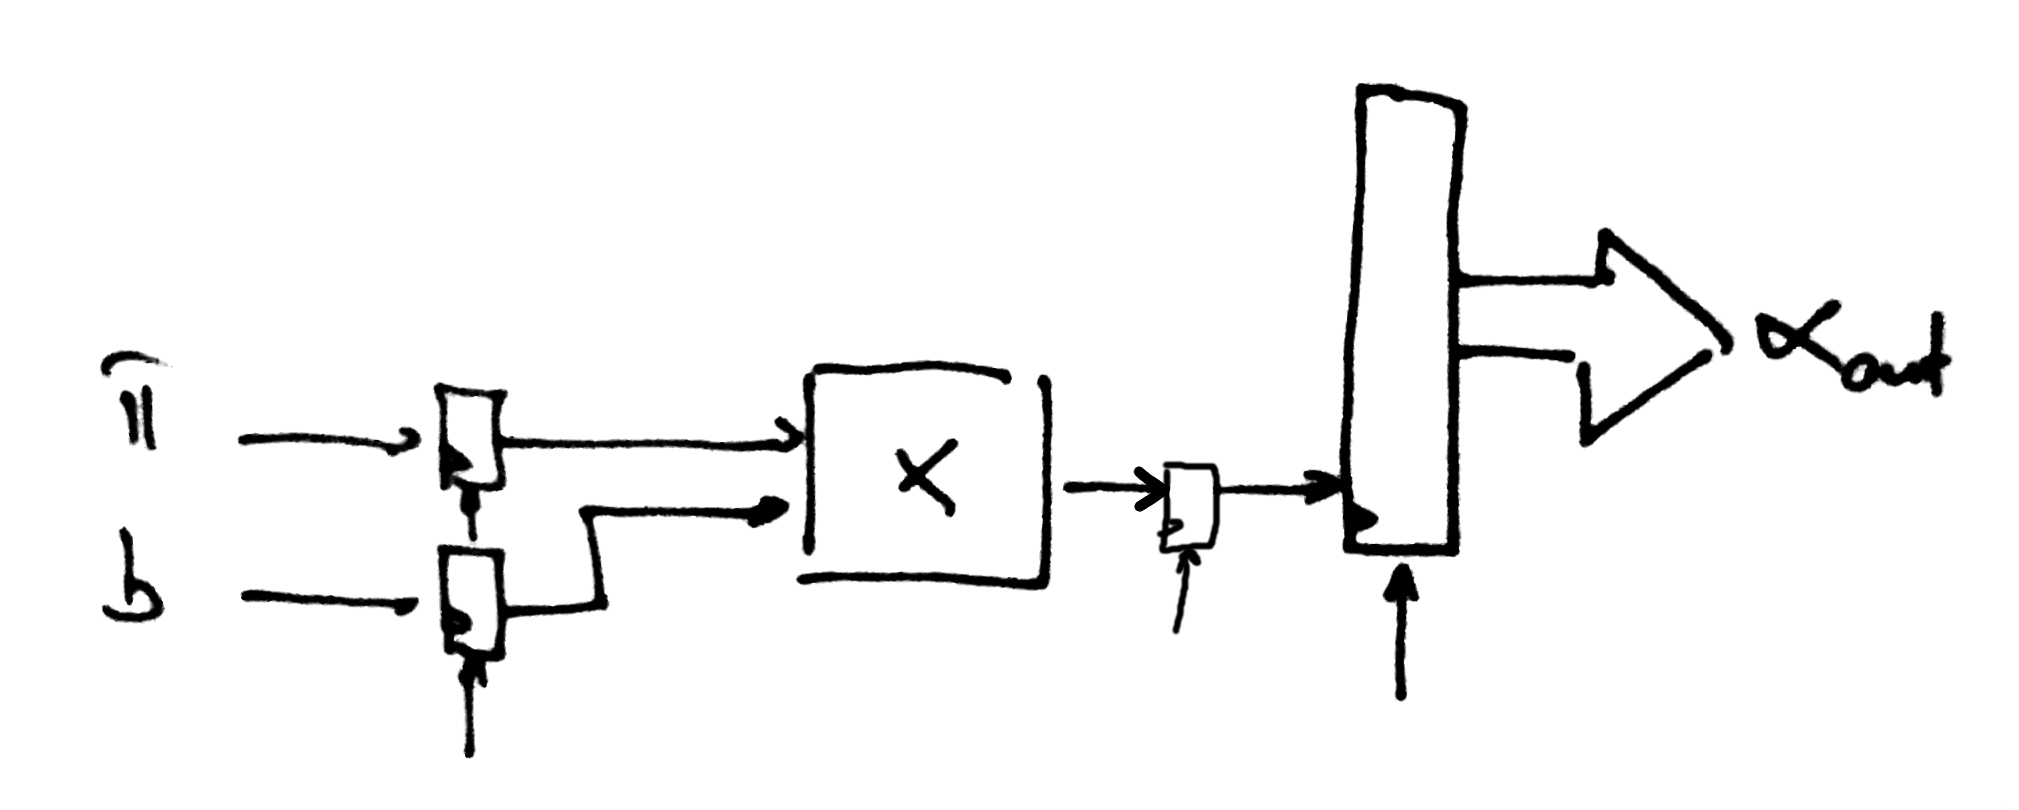
\includegraphics[width=1\columnwidth]{./schema/arch_init_s.png}
    \caption{Initialisation step with one MACC}
    \label{fig:init_s}
\end{figure}

%-------------------------------------------------------------------------------
%===============================================================================
\section{k-th Forward Variable}
\emph{\color{red}better title?}

\begin{itemize}
    \item one pipelined MACC for the computation of all elements
    \item $ N $ pipelined MACC, each computing one $ \alpha_k $
    \item use optimized Matrix-Vector-Vector multiplication
        $ \alpha_{k+1} = TP * \alpha_k * B(o_k) $
        \cite{FCCM12_Kestur, ITNG07_Yang}
\end{itemize}

\begin{figure}
    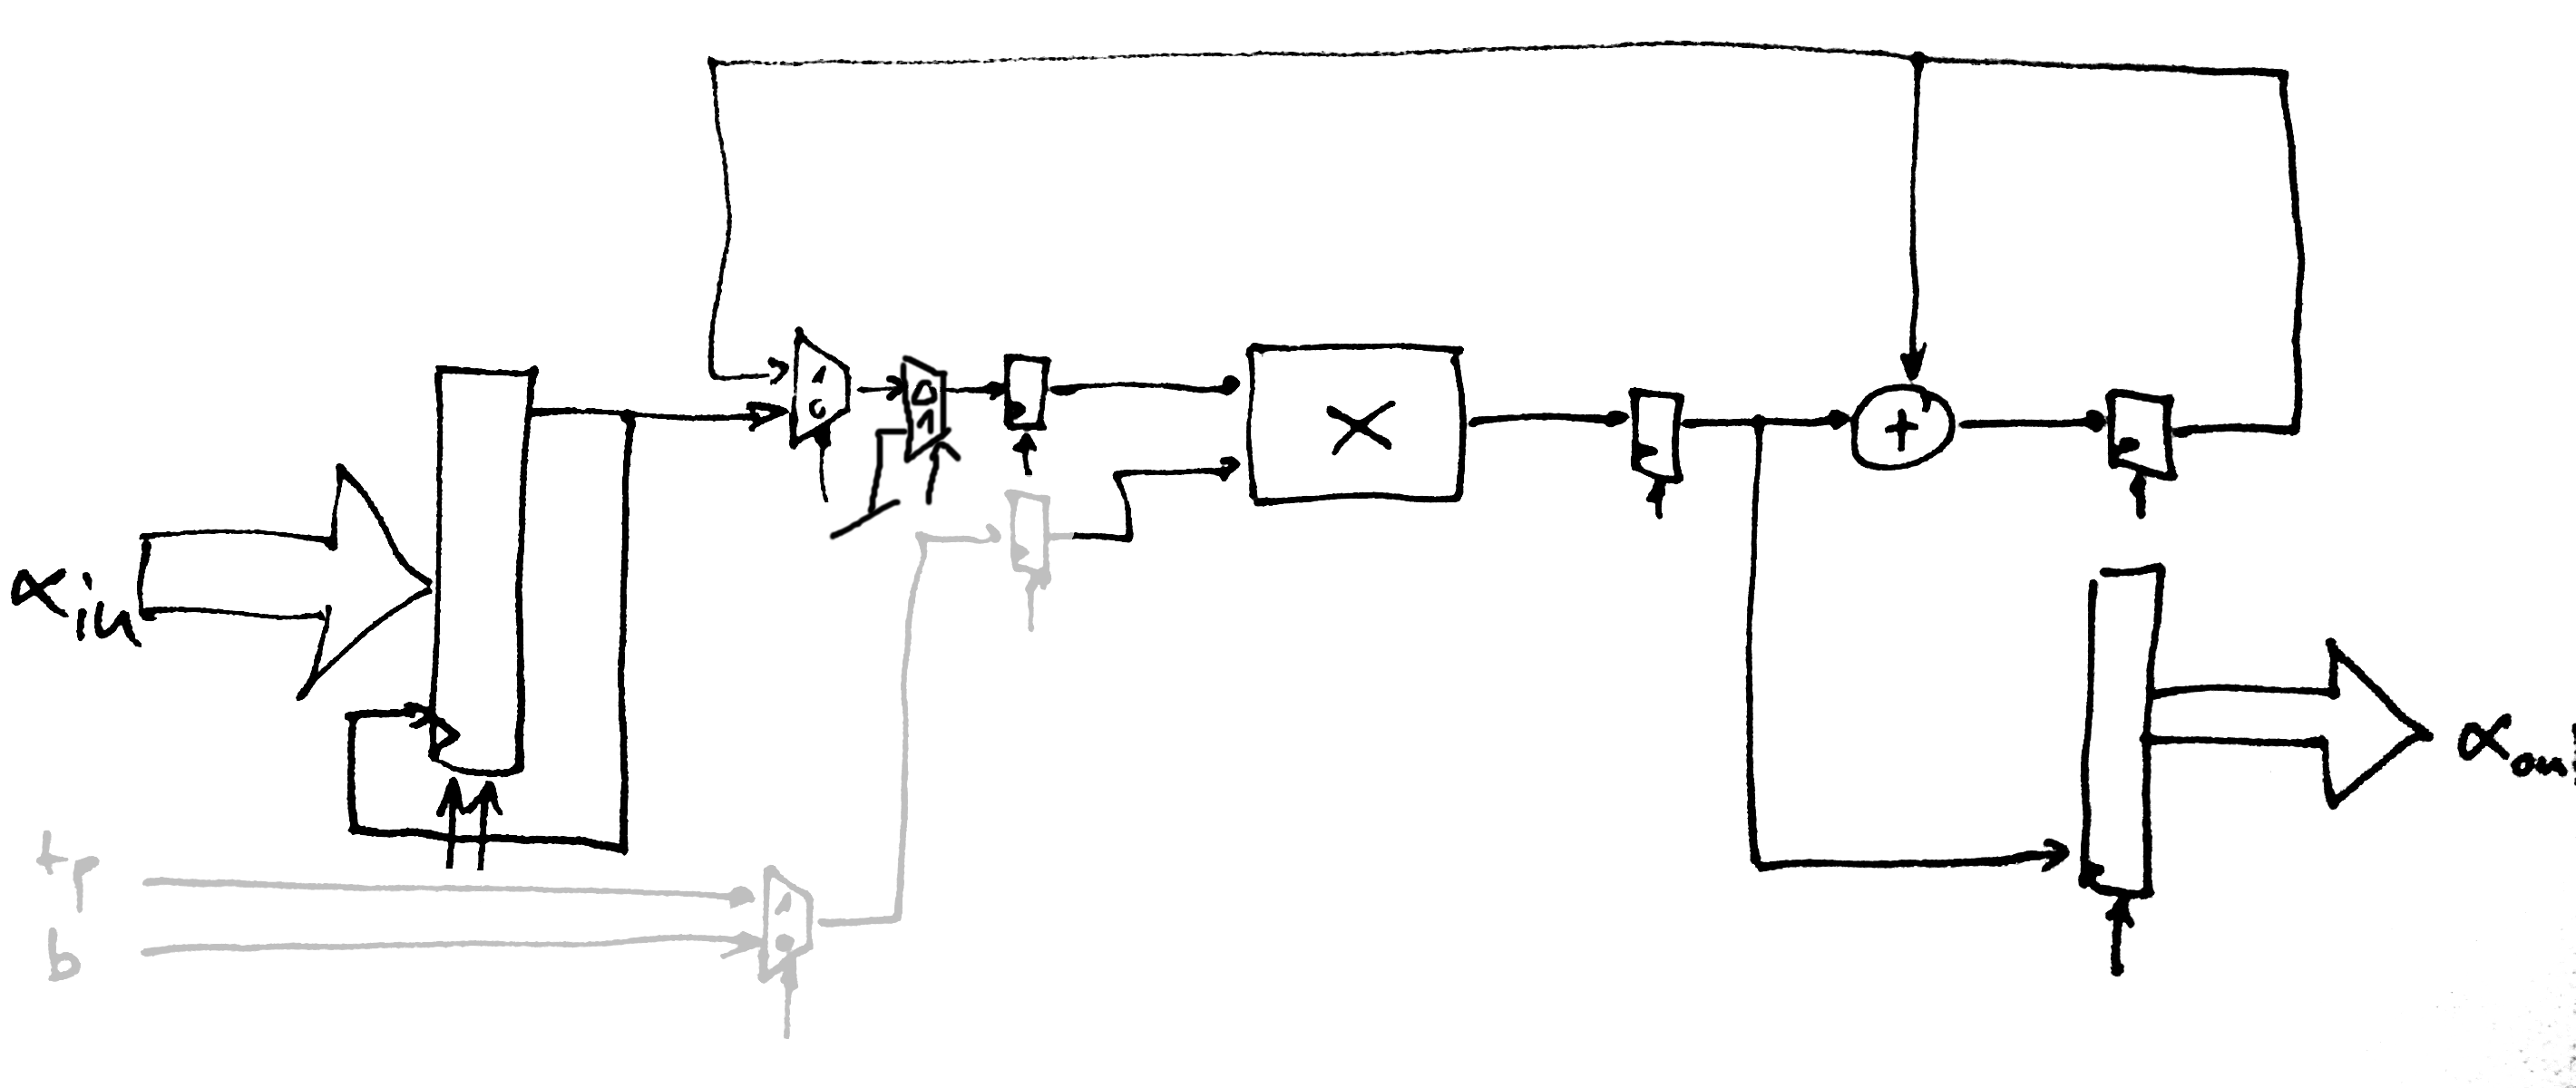
\includegraphics[width=1\columnwidth]{./schema/arch_step_s.png}
    \caption{k-th step with one MACC unit}
    \label{fig:step_s}
\end{figure}
\begin{figure}
    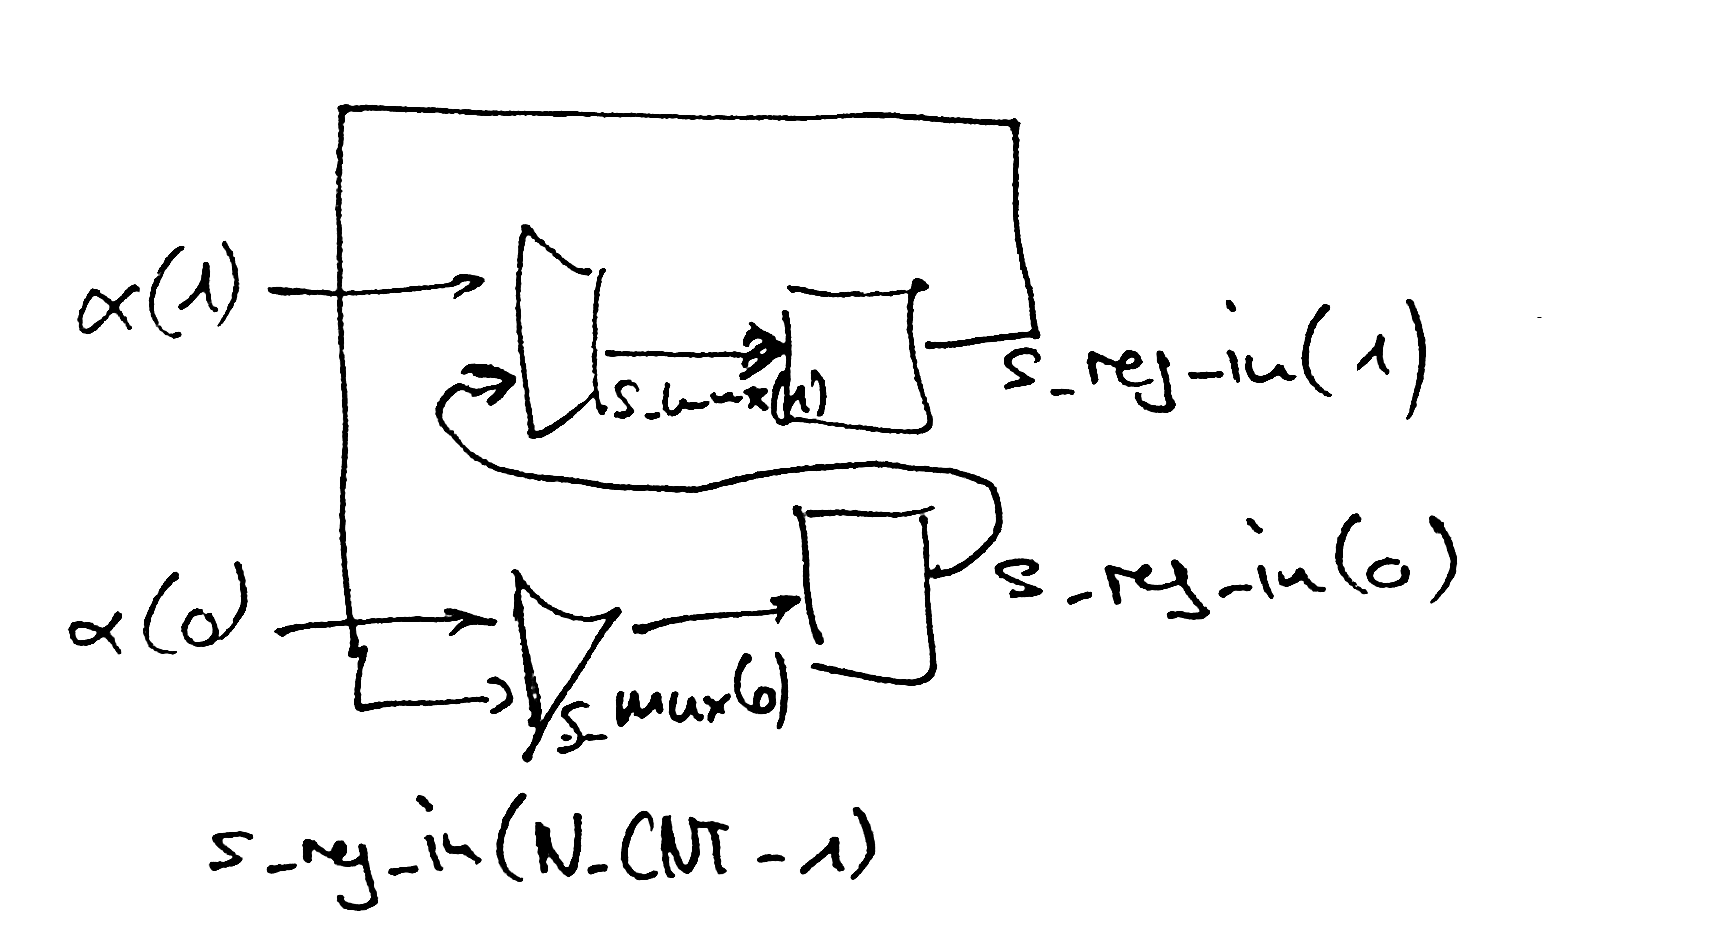
\includegraphics[width=1\columnwidth]{./schema/arch_shift_reg_s.png}
    \caption{Example of input shift register with N=2}
    \label{fig:shift_reg_s}
\end{figure}

\begin{figure}
    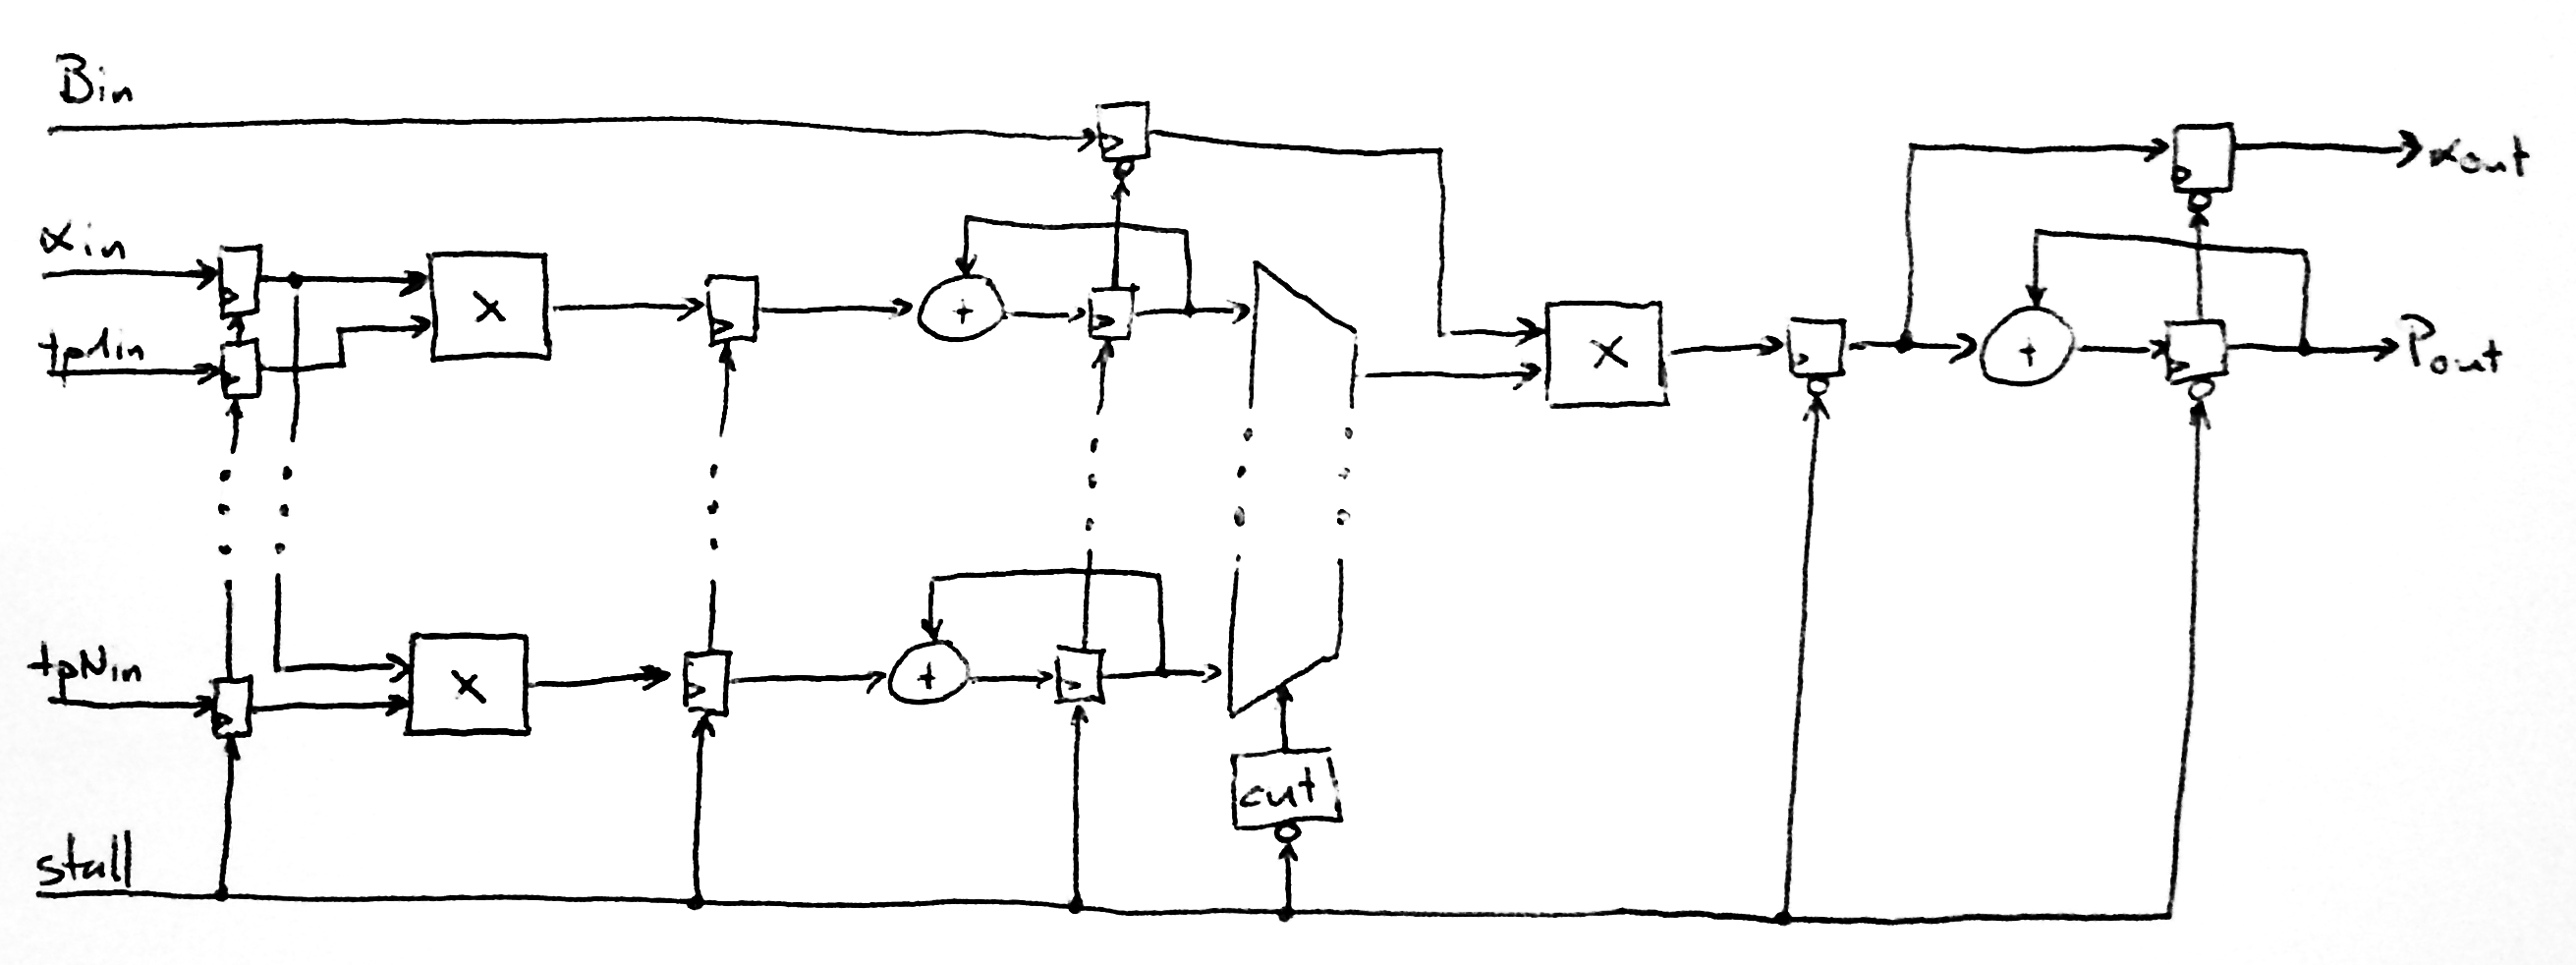
\includegraphics[width=1\columnwidth]{./schema/arch_step_p.png}
    \caption{k-th step with $ N+1 $ MACC units and integrated computation of P
        (which is only needed at the last step)}
    \label{fig:step_p}
\end{figure}

%-------------------------------------------------------------------------------
%===============================================================================
\section{Serial Controller}

\begin{figure}
    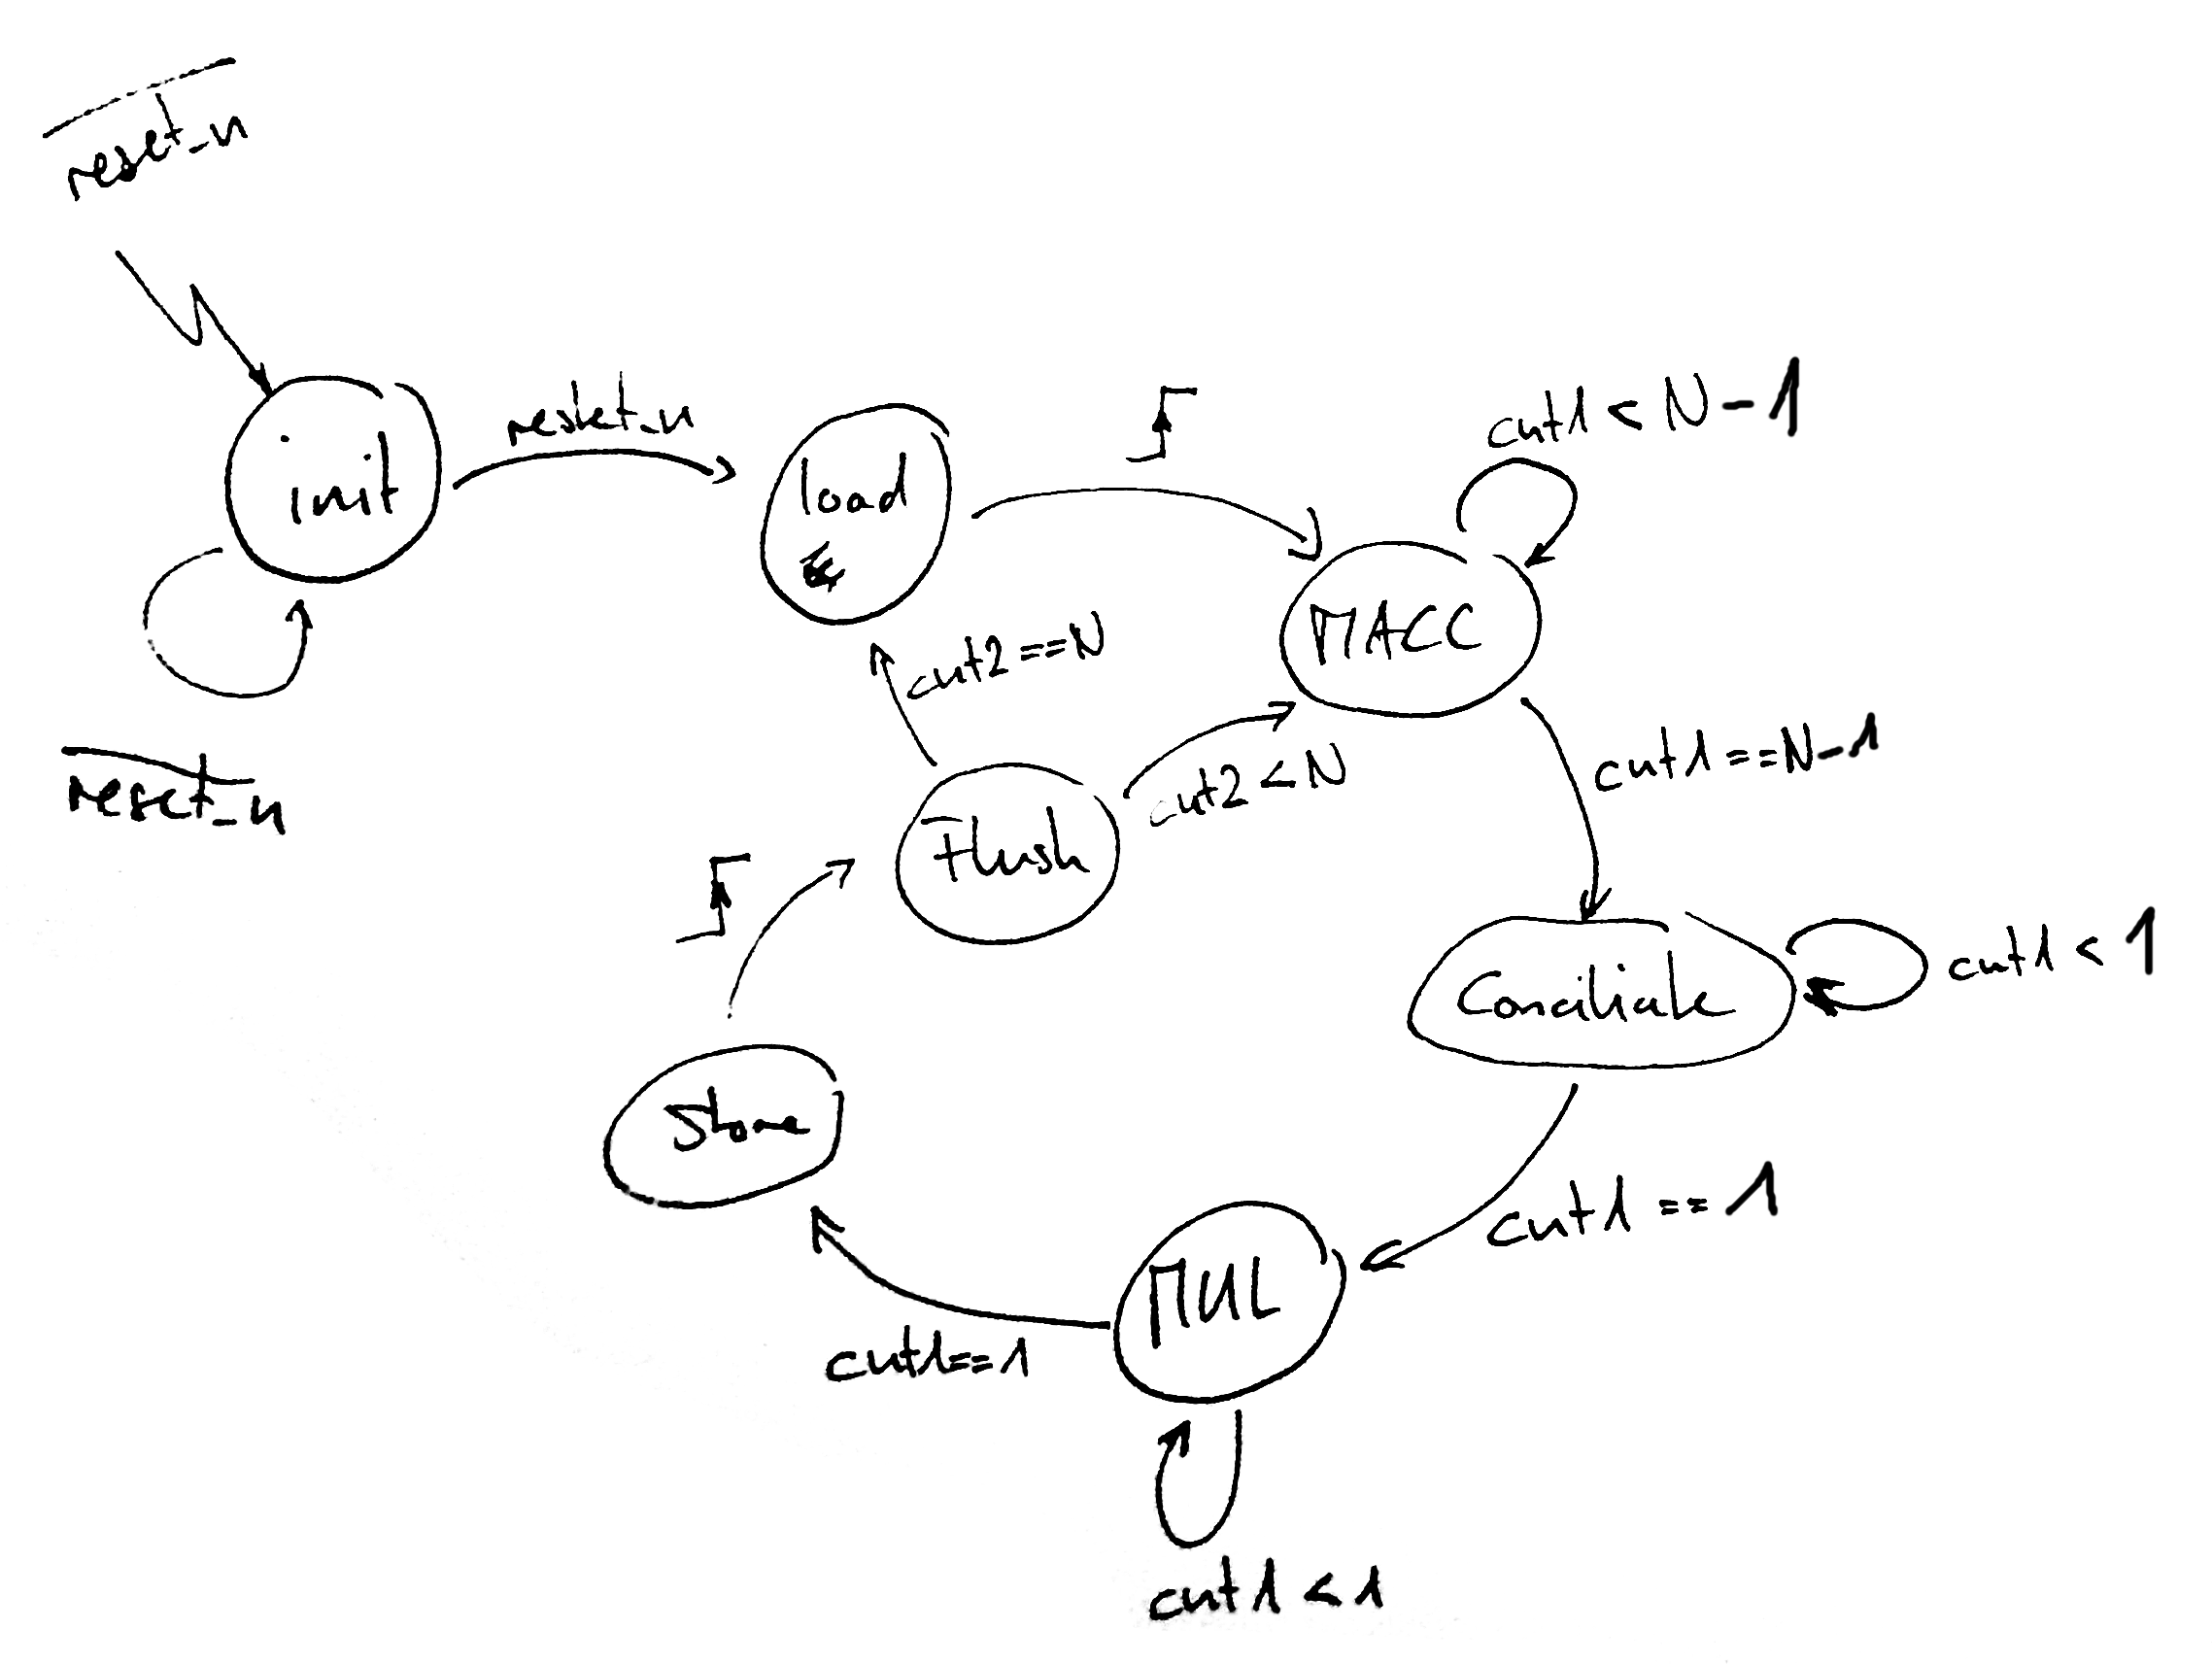
\includegraphics[width=1\columnwidth]{./schema/arch_ctrl.png}
    \caption{Controller of serial implementation}
    \label{fig:ctrl}
\end{figure}

\emph{\color{red} in table \ref{tab:ctrl} the signals flush\_Ps and load\_out
are only set in the first iteration. Add a footnote?}

\begin{table}
    \begin{center}
    \begin{tabular}{|l|c|c|c|c|c|c|c|}
    \hline
                      & INIT & SELECT & MACC & CONCILIATE & MUL & STORE & FLUSH \\
    \hline
    shift\_alpha\_in  & 0    & 0      & 1    & 0          & 0   & 0     & 0     \\
    shift\_alpha\_out & 0    & 0      & 0    & 0          & 0   & 1     & 0     \\
    conciliate        & 0    & 0      & 0    & 1          & 0   & 0     & 0     \\
    enable\_init      & 0    & 0      & 0    & 0          & 1   & 0     & 0     \\
    enable\_step      & 0    & 0      & 1    & 1          & 1   & 0     & 0     \\
    enable\_final     & 0    & 1      & 0    & 0          & 0   & 0     & 0     \\
    flush             & 0    & 0      & 0    & 0          & 0   & 0     & 1     \\
    \hline
    \end{tabular}
    \end{center}
    \caption{Control signals}
    \label{tab:ctrl}
\end{table}

%-------------------------------------------------------------------------------
%===============================================================================
\section{Balancing Pipeline Stages}

%-------------------------------------------------------------------------------
%===============================================================================
\section{Practical Notes}

\begin{itemize}
    \item generic design (change N, L and bit widths in param\_pkg)
    \item if bit widths of op1 is changed, fifo\_512x25 must be regenerated
\end{itemize}

%===============================================================================
%%%%%%%%%%%%%%%%%%%%%%%%%%%%%%%%%%%%%%%%%%%%%%%%%%%%%%%%%%%%%%%%%%%%%%%%%%%%%%%%
\chapter{Testing and Verification}
\label{ch:test}

%-------------------------------------------------------------------------------
%===============================================================================
\section{Device}
\label{ch:test_dev}

\begin{itemize}
    \item Nexys4 board with Artix-7 FPGA
    \item limited recourses -> proof of concept
    \item bord hardware for testing
\end{itemize}

%-------------------------------------------------------------------------------
%===============================================================================
\section{Relation to Proposed Algorithm}
\label{ch:test_prop}

%-------------------------------------------------------------------------------
\subsection{Log Standard}

%-------------------------------------------------------------------------------
\subsection{Metrics}

%===============================================================================
%%%%%%%%%%%%%%%%%%%%%%%%%%%%%%%%%%%%%%%%%%%%%%%%%%%%%%%%%%%%%%%%%%%%%%%%%%%%%%%%
\chapter{Results}
\label{ch:res}
%-------------------------------------------------------------------------------
\section{Speedup}
\label{ch:res_speed}
%-------------------------------------------------------------------------------
\section{Accuracy}
\label{ch:res_prec}

%===============================================================================
%%%%%%%%%%%%%%%%%%%%%%%%%%%%%%%%%%%%%%%%%%%%%%%%%%%%%%%%%%%%%%%%%%%%%%%%%%%%%%%%
\chapter{Conclusion}
\label{ch:conc}

%-------------------------------------------------------------------------------
%===============================================================================
\section{Achievements}
\label{ch:conc_ach}

%-------------------------------------------------------------------------------
%===============================================================================
\section{Future Work}
\label{ch:conc_work}

\nocite{*}

\appendix %optional, use only if you have an appendix

%===============================================================================
%%%%%%%%%%%%%%%%%%%%%%%%%%%%%%%%%%%%%%%%%%%%%%%%%%%%%%%%%%%%%%%%%%%%%%%%%%%%%%%%
\chapter{Some material}
%\section{It's over\dots}

\backmatter

%\chapter{Glossary} %optional

%\bibliographystyle{alpha}
%\bibliographystyle{dcu}
%\bibliographystyle{plainnat}
%\bibliographystyle{plain}
%\bibliographystyle{abbrvnat}
\bibliographystyle{siam}
%\bibliographystyle{ieeetr}
\bibliography{biblio}

%\cleardoublepage
%\theindex %optional, use only if you have an index, must use
	  %\makeindex in the preamble

\end{document}
